\chapter{Grundlagen}
\label{sec:grundlagen}

\section{Grid Fins als Steuerelement von Flugkörpern im Hyperschall}
\subsection{Aufbau}
Um Grid Fins und ihre Orientierung beschreiben zu können, werden zunächst einige Größe eingeführt.
In der simpelsten Konfiguration bestehen Grid Fins aus einem äußeren Rahmen, der die innere Struktur von sich kreuzenden planaren Flächen stützt. Dieser einfache Aufbau gewährt hohe Stabilität bei vergleichsweise geringem Gewicht \cite{zellform} und lässt sich mittels 5 Parameter, wie in Abbildung \ref{abb_parameter} zu sehen, beschreiben. Die Wanddicke $\gls{symb:d}$ kann sich für den Rahmen ($d_{\gls{Index:R}}$) von der des Gitters ($d_{\gls{Index:G}}$) unterscheiden. Aber auch innerhalb dieser Einteilung kann der Wert variieren. So ist häufig die Wandstärke in der Nähe der Einspannung erhöht, um die dort auftretenden höheren Beanspruchungen zu ertragen. Ein von den Wänden umrahmter Durchlass des Gitters wird als Zelle bezeichnet und seine Abmessung kann mit die Zellgröße $\gls{symb:g}$ beschrieben werden. Die Ausmaße der Grid Fins werden maßgeblich durch die Spannweite $\gls{symb:b}$ und die Höhe $\gls{symb:h}$ bestimmt. Die Querschnittsfläche $\gls{symb:A}$ steht in der Ausgangsstellung senkrecht zur Anströmung und wird vom Rahmen begrenzt. Normal zu dieser Fläche steht die Sehne mit einer im Vergleich zur planaren Finne deutlich kürzeren Länge $\gls{symb:s}$.\\
\begin{figure}[h]
	\centering
	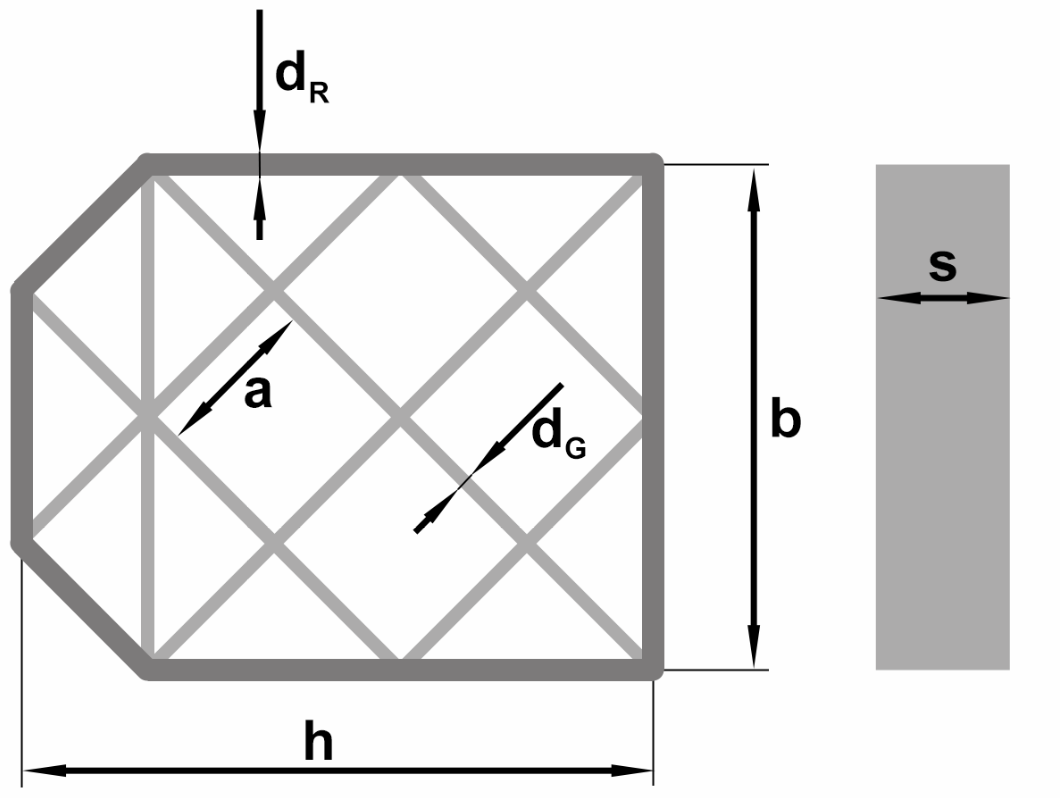
\includegraphics[width=0.6\textwidth]{Parameter.png}
	\caption{Aufbau eines einfachen Grid Fins}
	\label{abb_parameter}
\end{figure}\\
Grid Fins müssen nicht starr an einem Flugkörper, zum Beispiel der Rakete, befestigt werden, sondern können um mehrere Achsen drehbar sein. Um sie für den Transport kompakt zu lagern, lassen sie sich an den Körper anlegen. Der Klappwinkel $\gls{symb:Lambda}$ beschreibt den Ausschlag um eine den Körper an der Anbringung tangierende Achse. Ein Klappwinkel von $0^\circ$ entspricht hierbei dem normalen in die Strömung ragenden Zustand und $90^\circ$ dem eingeklappten. Zur Steuerung lassen sich die Grid Fins um eine Achse, die orthogonal aus dem Körperoberfläche durch die Mitte des Grid Fins zeigt, verstellen. Ein Steuerwinkel von $\eta = 0^\circ$ ist auch hier wieder die Ausgangsstellung, die Sehne ist parallel zur X-Achse. Bei $\eta = 90^\circ$ würde also die Seitenkante zur Anströmung zeigen. Die Querschnittsfläche $A$ und somit also auch das Gitter wird nicht durchströmt.
\begin{figure}[h]
	\centering
	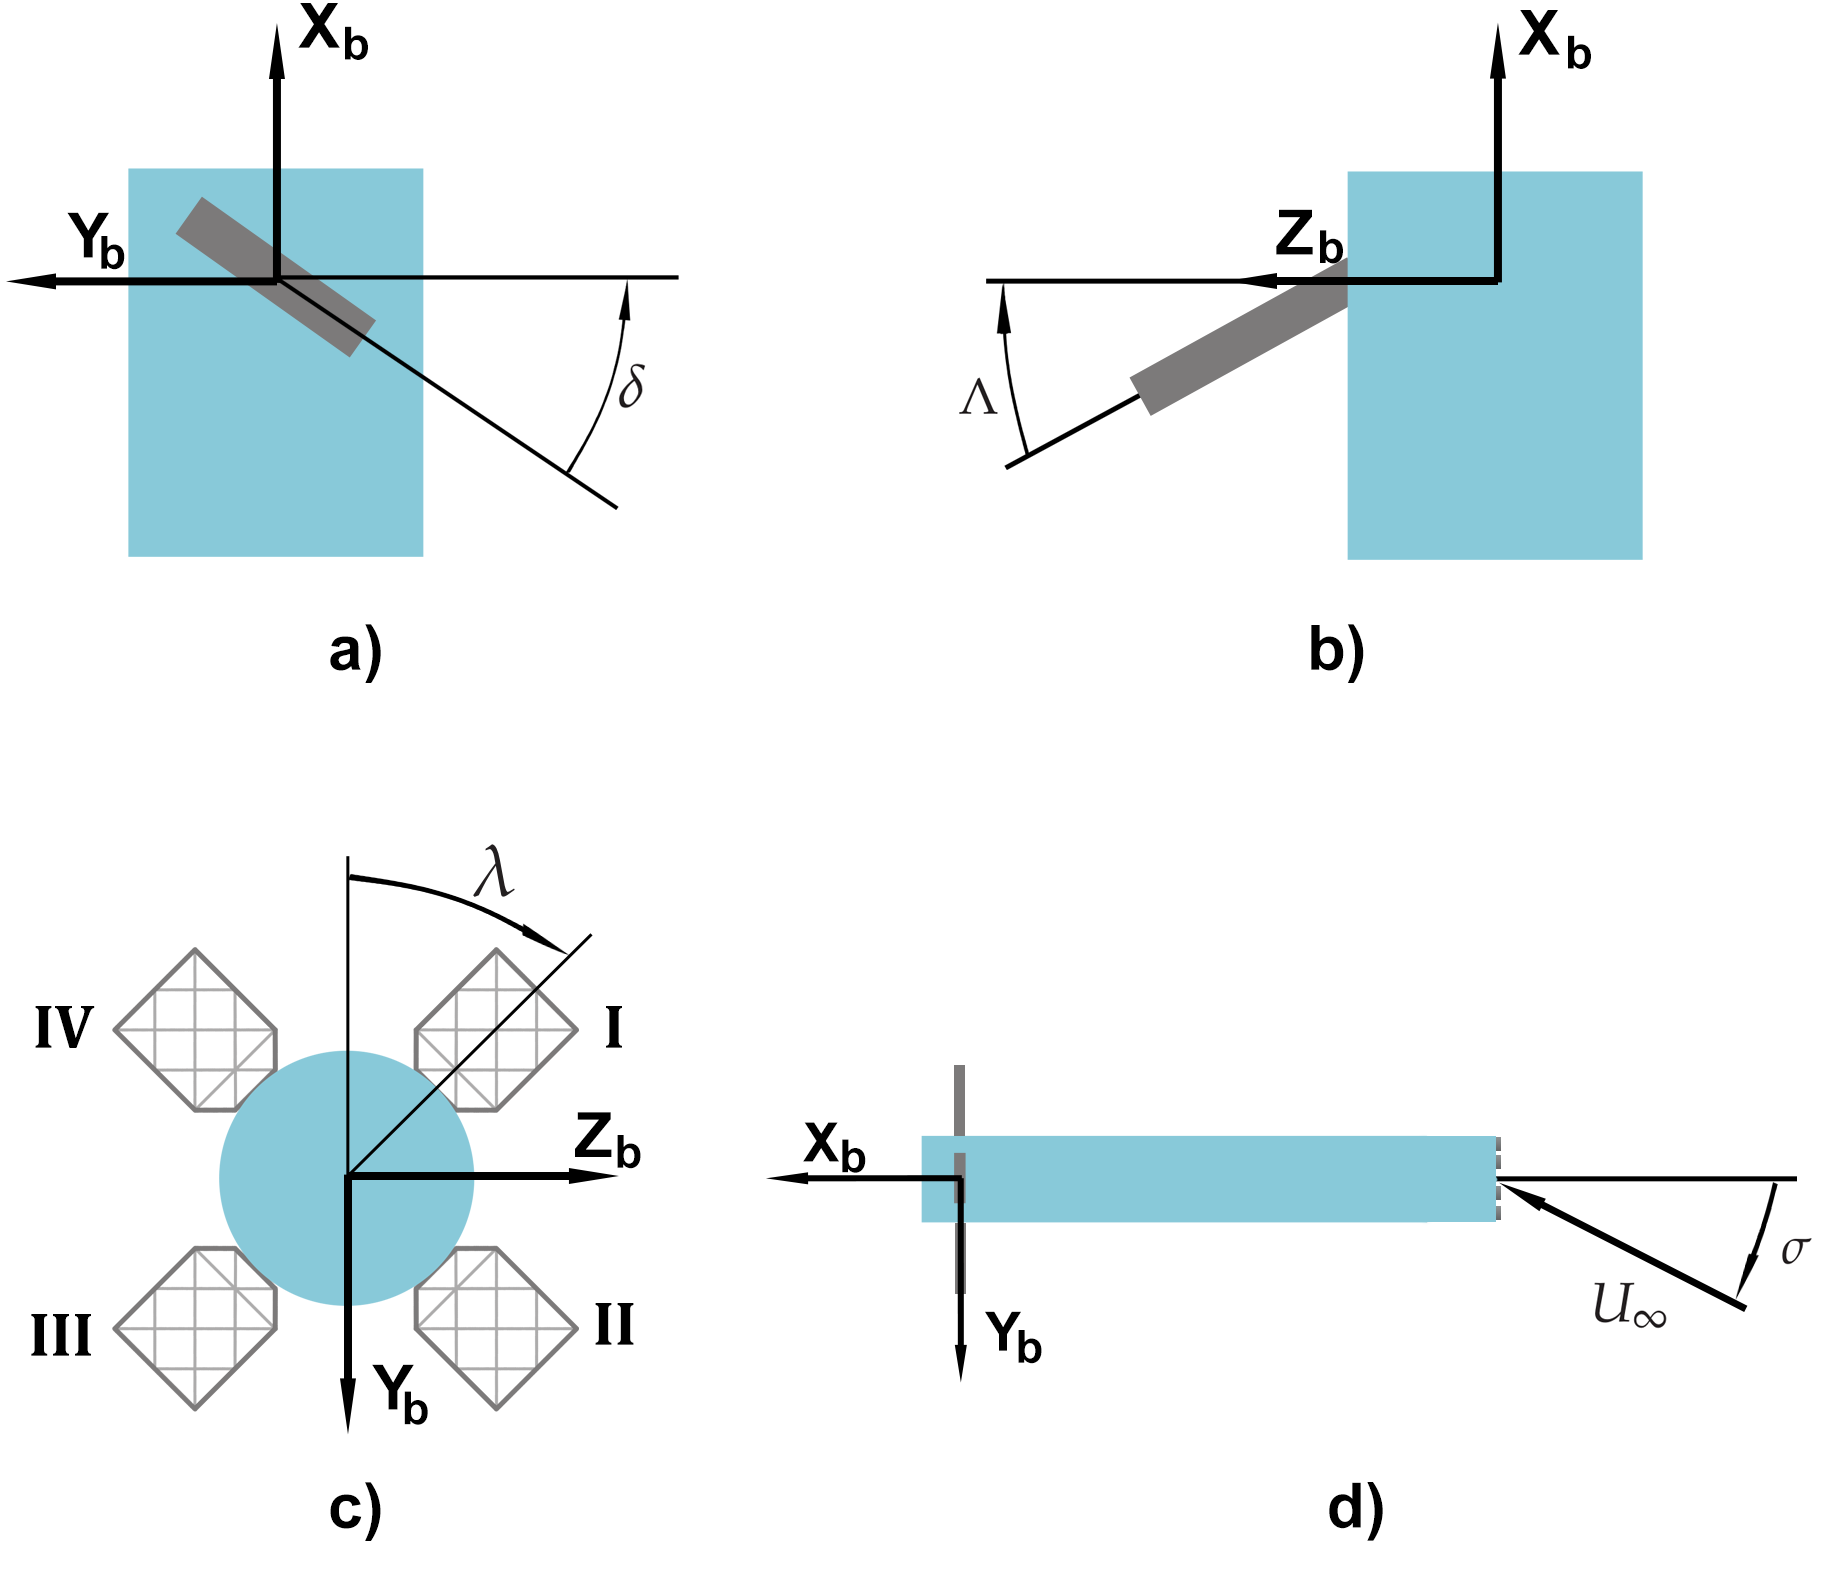
\includegraphics[width=0.8\textwidth]{Winkel.png}
	\caption{Winkel zur Beschreibung der Orientierung der Grid Fins zum Körper\\a) Steuerwinkel, b) Klappwinkel, c) Drehwinkel, d) Neigungswinkel des Körpers zur Anströmung}
	\label{abb_winkel}
\end{figure}\\
Um die Aerodynamik zu untersuchen reichen diese Winkel nicht aus, da die Anströmung nicht parallel zur Rakete liegen muss. Der Neigungswinkel des gesamten Moduls zur Anströmung $\gls{symb:sigma}$ setzt sich unter realen Bedingungen mit Vernachlässigung des Windes aus dem Schiebewinkel und dem Bahnneigungswinkel zusammen. Für die in dieser Arbeit durchgeführten Untersuchungen ist eine solche Aufteilung aber irrelevant. Damit aber keine Informationen und somit Genauigkeit verloren geht, wird stattdessen die Orientierung der Grid Fins auf dem Umfang betrachtet. Verwendet wird hier eine Anordnung von vier gleichmäßig verteilten Steuerelementen. Das Koordinatensystem ist so definiert, dass es seinen Ursprung genau in der Mitte dieser Konfiguration hat und die positive X-Achse zur Spitze des Flugkörpers, also entgegen der Anströmung, zeigt. Bei $\sigma \neq 0$ zeigt auch die Y-Achse einem Anteil der Strömung entgegen. Die Z-Achse ist folglich nach dem Rechtssystem orthogonal zu den anderen beiden ausgerichtet. Um nun die Orientierung der Grid Fins um die X-Achse herum beschreiben zu können wird der Rollwinkel $\gls{symb:lambda}$ eingeführt. Wenn eine '+'-Konfiguration vorliegt, befinden sich die einzelnen Finnen auf den Koordinatenachsen (X, Y) und der Rollwinkel ist gleich null. Im Gegensatz dazu sind sie bei der 'x'-Konfiguration um einen Winkel von $\lambda = 45^\circ$ verdreht. Der Anstellwinkel $\gls{symb:alpha}$, den ein einzelner Grid Fin erfährt, lässt sich aus dem Neigungswinkel des Körpers und, in Abhängigkeit vom Rollwinkel und welcher der Finnen betrachtet wird, aus dem Klapp- und Steuerwinkel bestimmen.


\subsection{Strömung durch Grid Fins}\label{stroe}
Um die Eigenschaften von Grid Fins analysieren zu können, ist es nötig die zugrunde liegenden strömungsmechanische Vorgänge zu verstehen. Dazu werden in diesem Abschnitt das Verhalten der Strömung im Unter-, Überschall und besonders auch im transsonischen Bereich mit Schwerpunkt auf Verdichtungsstöße besprochen.
Bei niedrigen Strömungsgeschwindigkeiten im Unterschall haben Grid Fins auf Grund ihrer geringen Dicke keinen großen Einfluss auf das Fluid, welches nahezu ungestört durch das Gitter fließen kann \cite{sb-sharp}. Mit steigenden Machzahlen tritt aber zunehmend der Effekt auf, dass die Strömung um die stumpfe Vorderkante des Gitters in die Zelle hinein expandiert. Zusammen mit der Grenzschichtbildung an den Zellwänden, die effektiv zu Verengung der durchströmten Fläche führt, wir die Strömung innerhalb der Zellen auf Geschwindigkeiten beschleunigt, die über der der Anströmung liegen \cite{synopsis}.
\begin{figure}[h]
	\centering
	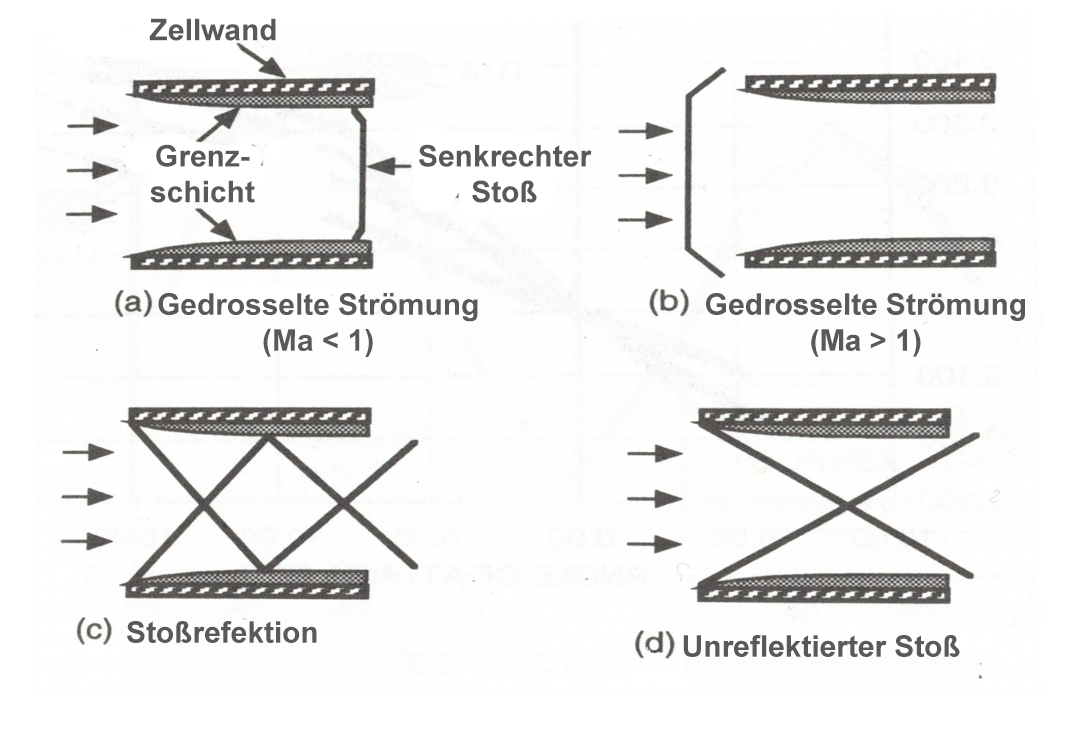
\includegraphics[width=0.7\textwidth]{swallow.png}
	\caption{Stoßsystem einer Zelle aus \cite{synopsis}}
\end{figure}\\

Der transsonische Bereich wird ab einer Anströmungsmachzahl von circa $Ma_\infty=0,8$ erreicht \cite{machgrenzen} und ist für die Aerodynamik der Grid Fins eine sehr kritische Problematik. Sobald die Strömung innerhalb des Gitters eine Machzahl von $1$ überschreitet, kommt es zu einem Verdichtungsstoß am Ausgang der Zellen, der mit steigender Machzahl an Stärke zunimmt. Dieser führt zu einer Drosselung der Strömung, was den Effekt hat, dass ein Teil der Strömung verdrängt wird und sich stattdessen um den Grid Fin herumbewegt. Steigt nun auch $Ma_{\gls{Index:inf}}$ über $1$ löst sich der Stoß von den Gitterwänden und verbindet sich zu einer unregelmäßigen 3D-Struktur in der Abströmung \cite{stroemung}. Wächst $Ma_\infty$ weiter an, so kommt es zu einem Verdichtungsstoß vor dem Grid Fin. Dies führt dazu, dass innerhalb der Zellen keine Drosselung mehr vorliegt \cite{stroemung}, stattdessen wird die Strömung schon durch den Stoß vor dem Gitter um dieses herum verdrängt \cite{synopsis}. Von den Vorderkanten gehen Schockwellen aus, die auf benachbarte Wände treffen und von ihnen reflektiert werden \cite{synopsis}. Steigt die Machzahl weiter an, so befinden sich diese Wellen auf steileren Bahnen bis sie gar nicht mehr auf die anderen Wände treffen. Des Weiteren nähert sich der Verdichtungsstoß vor dem Grid Fin diesem immer weiter mit größer werdenden Strömungsgeschwindigkeiten an, bis es abgesehen von der direkten Umgebung der Wände gar nicht mehr zum Stoß kommt. Die einzelnen Zellen fungieren nun als Überschalldüse \cite{stroemung}, sodass die Strömung in den meisten Bereichen nicht mehr auf den Unterschall abgebremst wird. Der Stoß wurde vom Gitter "verschluckt".
\\~\\
Als ein besonderer Bereich ist noch die Ansatzregion zu betrachten, in der der Grid Fin an der Rakete angebracht ist. Schnittstellen von Wänden stellen ein erhöhtes Potenzial für blockierte Strömung dar. In der Ansatzregion befinden sich nicht nur vielen von diesen Schnittstellen, sondern auch die Wanddicke ist hier meistens am größten. Dies in Kombination mit einer schon durch die Grenzschichtwirkung des Körpers verzögerte Strömung, führt zu einer relativ großen Region verlangsamter Strömung oder gar Rückströmung, die mit der Machzahl an Größe gewinnt \cite{stroemung}. Bei einer Machzahl von ungefähr $Ma_\infty = 2$ erreicht diese jedoch ein Maximum, da die Strömung bei weiter steigenden Geschwindigkeiten von der umgebenden mitgerissen wird und diese Region somit wieder an Größe und Bedeutung verliert \cite{stroemung}.

Es ist nun also hervorzuheben, dass Grid Fins weder im Unterschall noch im hohen Überschall übermäßig starke Störungen der Strömung bewirken. Im transsonischen Bereich jedoch kommt es zu massiven Verdichtungsstößen, die zu einer starken Drosselung des Fluids führen.


\subsection{Aerodynamische Beiwerte und Vergleich zu planaren Finnen}
Nachdem nun die zugrunde liegende Strömung verstanden ist und Größen zur Beschreibung von Grid Fins etabliert wurden, werden nun die aerodynamischen Kräfte beschrieben. Hierbei wird der Vergleich zu den konventionellen planaren Finnen gezogen.
\begin{figure}[h]
	\centering
	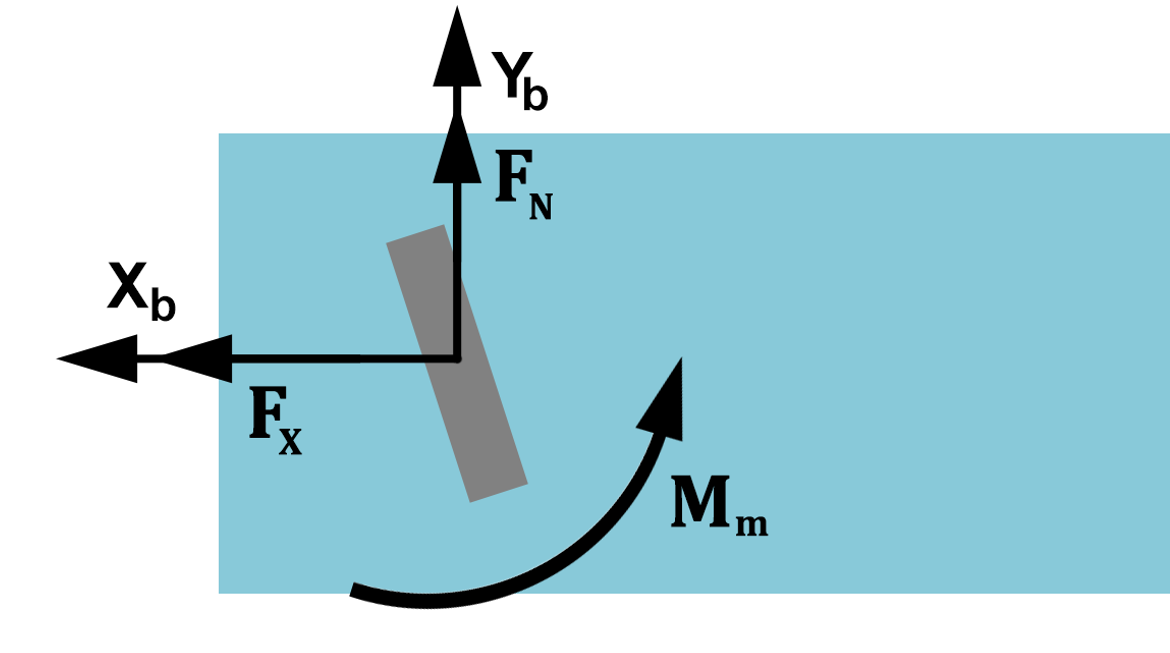
\includegraphics[width=0.6\textwidth]{kraefte.png}
	\caption{Kräfte und Momente am Grid Fin}
\end{figure}\\
Relevant sind zum einen die Kräfte, die normal zur X-Achse, also in der X-Y-Ebene, liegen ($\gls{symb:F}_{\gls{Index:N}}$) und zum anderen die Kräfte, die in negative X-Richtung zeigen $F_{\gls{Index:X}}$. Bei einem Neigungswinkel von $\sigma = 0$ entsprechen sie dem Auftrieb und Widerstand. Zusätzlich ist auch noch das Moment $\gls{symb:M}_{\gls{Index:m}}$ um die Achse in der die Grid Fins steuerbar gelagert ist relevant.
\subsubsection{Normalkraft}
Die Normalkrafterzeugung ist ausschlaggebend für die Stabilität und Steuerbarkeit eines Flugkörpers. Die Steigung der Normalkraftkoeffizient über den Anstellwinkel $\gls{symb:C}_{N\alpha}$ bei einem Anstellwinkel von $\alpha = 0$ ist in Abbildung \ref{abb_bucket} zu sehen. Wie in Abschnitt \ref{stroe} beschrieben, führt die Drosselung im transsonischen Bereich dazu, dass die Strömung um den Grid Fin herum verdrängt wird. Dadurch büßt er einen nicht vernachlässigbaren Teil seiner Fähigkeit Normalkraft zu erzeugen ein. Dieser Effekt ist genau gegensätzlich zu konventionalen planaren Finnen, die im Transschall ihren maximalen Normalkraftkoeffizienten $C_N$ erreichen \cite{synopsis}.
\begin{figure}[h]
	\centering
	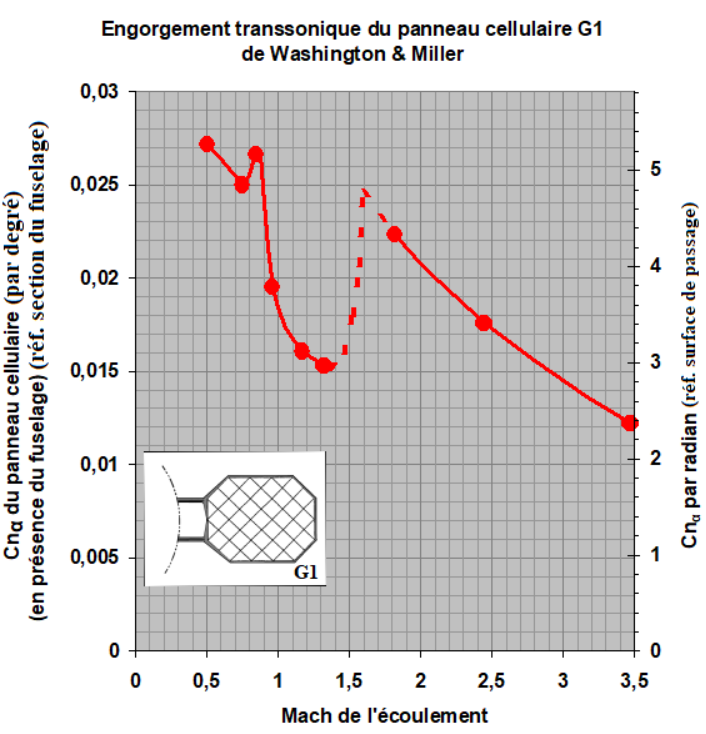
\includegraphics[width=0.6\textwidth]{bucket.png}
	\caption{Normalkraftsbeiwertgradient bei $\alpha = 0$ über die Machzahl aus \cite{synopsis}}
	\label{abb_bucket}
\end{figure}\\
Während vergleichbare konventionelle Finnen im Unterschall und niedrigen Überschall ähnlich hohe Normalkräfte erzeugen können, werden sie im hohen Machbereich von Grid Fins übertroffen. Schon ab $Ma=2,5$ kann die Normalkraft das 1,5-fache betragen und dieser Wert steigt mit der Machzahl nur noch weiter an \cite{synopsis,vergleichPlanarNATO}.
\subsubsection{Axialkraft}
Die Axialkraft wird häufig als der größte Nachteil angesehen, auch wenn der sich für spezielle Anwendungen als \grqq drag brake\grqq \ nutzen lässt. Wie schon im Abschnitt \ref{stroe} erwähnt, wird die Strömung bei niedrigen Geschwindigkeiten nicht stark gestört, folglich kommt es auch nicht zu großen Axialkräften. Im transsonischen Bereich steigt der Beiwert durch die Drosselung der Verdichtungsstöße rasant an und erreicht bei einer Machzahl knapp unter 1 sein Maximum \cite{solver}. Danach nimmt der Wert wieder ab und bleibt im Überschall nahezu konstant, während er für planare Finnen abnimmt \cite{vergleichPlanarNATO}. Generell kann die Axialkraft von Grid Fins das bis zu drei- oder  vierfache des konventionellen betragen.
\begin{figure}[h]
	\begin{minipage}[t]{0.45\linewidth}
		\centering
		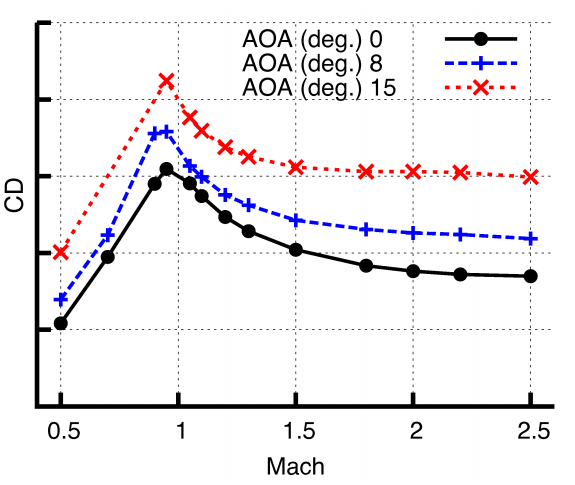
\includegraphics[width=0.945\textwidth]{Cd-Ma.png}
		\caption{Axialkraft (hier CD) bei unterschiedlichen Anstellwinkeln über Ma aus \cite{solver}}
	\end{minipage}
	\hfill
	\begin{minipage}[t]{0.45\linewidth}
		\centering
		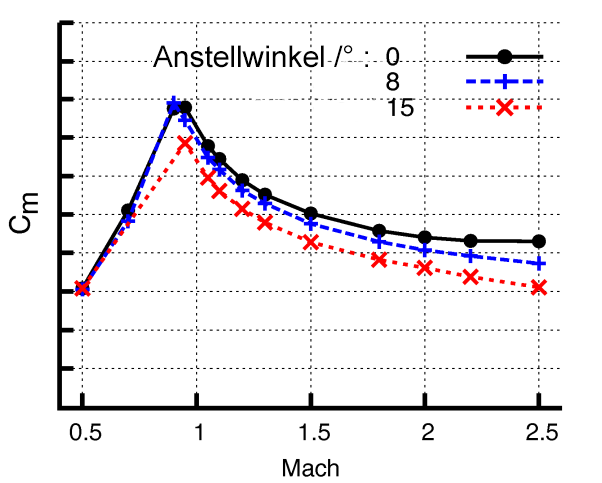
\includegraphics[width=\textwidth]{gelenkmomentMa.png}
		\caption{Gelenkmomentenbeiwert bei unterschiedlichen Anstellwinkeln über Ma aus \cite{solver}}
		\label{abb_Mm-Ma}
	\end{minipage}
\end{figure}\\
\subsubsection{Gelenkmoment}
Ein großer Vorteil von Grid Fins ist ihr geringes Moment um das Steuergelenk, welches den Einsatz von kleineren, weniger leistungsstarken Aktuatoren ermöglicht. Was wiederum eine Einsparung an Gewicht und Kosten mit sich bringt. Der Grund für das niedrige Moment ist hauptsächlich die im Vergleich zur planaren Finne deutlich kürzere Sehne, die der Luftkraft nur einen kleinen Hebelarm bietet. Der Druckpunkt befindet sich schon bei niedrigen Machzahlen in der Nähe der Mitte der Sehne, die die Achse ist, um die der Grid Fin gedreht wird, und wandert mit steigender Machzahl wenn auch nur leicht weiter Richtung 50\% der Sehnenlänge \cite{vergleichPlanarNATO}. Dies führt dazu, dass das Gelenkmomentbeiwert $C_m$ mit steigender Machzahl abnimmt. Ebenso wie bei der Axialkraft befindet sich das Maximum bei Machzahlen knapp unter 1, wie in Abbildung \ref{abb_Mm-Ma} zu sehen. Auch für Variationen des Anstellwinkels beleibt der Beiwert durchgehend auf einem niedrigen Niveau, deutlich unter dem seines planaren Gegenstücks \cite{vergleichPlanarNATO}. Es sei hier jedoch anzumerken, dass es möglich ist eine planare Steuerfläche mit einem geringeren Moment zu erhalten, indem die Gelenkachse durch den Druckpunkt gelegt wird. Durch die große Druckpunktwanderung ist dies aber nur für einen kleinen vorher gewählten Machzahlengebiet dem Grid Fin überlegen, der über einen großen Geschwindigkeitsgebiet konstant gute Charakteristiken bietet.
\subsubsection{Stabilität}
Für die statische Stabilität eines Flugkörpers muss bei Neigungswinkeln $\sigma \neq 0$ ein Moment um den \gls{SP} entstehen, das die Orientierung der Körperachse wieder parallel zur Strömung ausrichtet. Grid Fins haben hier einen entscheidenden Vorteil gegenüber planaren Alternativen, da bei ihnen auch die Finnen, die bei einem Rollwinkel von $\lambda = 0$ vertikal ausgerichtet sind, zu diesem Moment beitragen. Selbst der Effekt von Wirbel auf die lee-Finne ist dadurch negiert, dass sich die Variation des lokalen Anstellwinkels über die vergleichsweise große durchströmte Querschnittsfläche ausgleicht. Somit tragen die vertikalen Grid Fins über den Machbereich mit ungefähr 30\% einen signifikanten Teil zur Stabilität bei \cite{vergleichPlanarNATO}. Das Rückstellmoment um den Schwerpunkt ist sowohl im Unterschall als auch im Überschall größer, nur im Transschall büßen auch hier die Kräfte wieder ein.

Die Steuerbarkeit, die Fähigkeit Momente zu generieren, die die Orientierung des Flugkörpers aus der stabilen Lage heraus verändern, ist dadurch aber leicht behindert. Wenn zwei gegenüberliegende Grid Fins einen Steuerwinkelausschlag erfahren und somit eine Normalkraft erzeugen, wirken die anderen beiden dieser Kraft mit den soeben angesprochenen 30\% entgegen.
\subsubsection{Anstellwinkelcharakteristika}
Im Gegensatz zu planaren Finnen, die bei hohen Anstellwinkeln Strömungsabriss erfahren, zeigen Grid Fins eine deutlich besseres Verhalten. Ihre kurze Sehne senkt die Gefahr der Strömungsablösung deutlich und erlaubt somit eine verlässlichere Normalkraftgenerierung, die sich auch noch bei hohen Anstellwinkeln steigern lässt. Somit liegt im Unterschall die maximale Normalkraft bei $\alpha = 40^\circ$ ohne jegliche Anzeichen von Strömungsabriss \cite{synopsis}.
Des Weiteren ist der Anstieg dieser Kraft mit dem Anstellwinkel im Überschall beinahe linear \cite{synopsis}, was eine sehr effektive Steuerung ermöglicht.\\
~\\
Die Axialkraft zeigt bei den meisten Machzahlen mit wachsendem Anstellwinkel ein ähnliches Verhalten wie die planaren Steuerflächen \cite{vergleichPlanarNATO}, deren Werte auch stark ansteigen.
\begin{figure}[h]
	\centering
	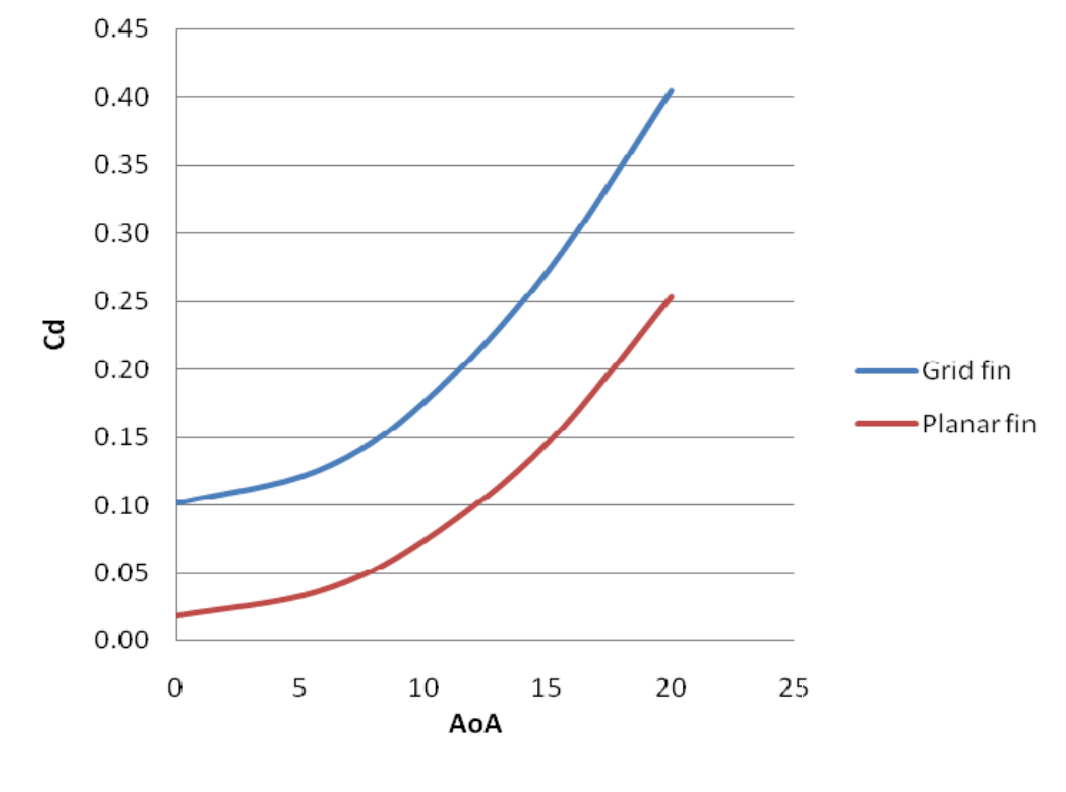
\includegraphics[width=0.5\textwidth]{Cd-AoA.png}
	\caption{Widerstandsbeiwert über Anstellwinkel bei $Ma=2,5$ aus \cite{vergleichPlanar}}
\end{figure}\\

In Bezug auf das Gelenkmoment $M_m$ zeigen Grid Fins wieder ein überlegendes Verhalten gegenüber planaren Finnen, wie in Abbildung \ref{abb_Mm-AoA} zu sehen. Während im Unterschall der Anstieg des Momentes nur geringfügig weniger steil ausfällt und für beide Steuerflächen ab einem Winkel von $\alpha \approx 10^\circ$bis$15^\circ$ zu stagnieren scheint, fällt der Unterschied im Überschall deutlich stärker aus. Die Kurve der planaren Finne zeigt einen rasanten Anstieg bei einer Anströmungsmachzahl von $Ma = 2,5$, die steigen des Grid Fins jedoch ist für niedrige Anstellwinkel fast noch auf dem selben Niveau, wie im Unterschall. Erst bei einem Anstellwinkel von circa $\alpha = 15^\circ$ nimmt auch hier die Steigung vergleichbare Werte an. Also ist die Steuerbarkeit bei hohen Machzahlen mit deutlich weniger Leistung möglich. Dies ermöglicht den Einsatz von bedeutend kleineren und somit auch kostengünstigeren Aktuatoren. 
\begin{figure}[h]
	\centering
	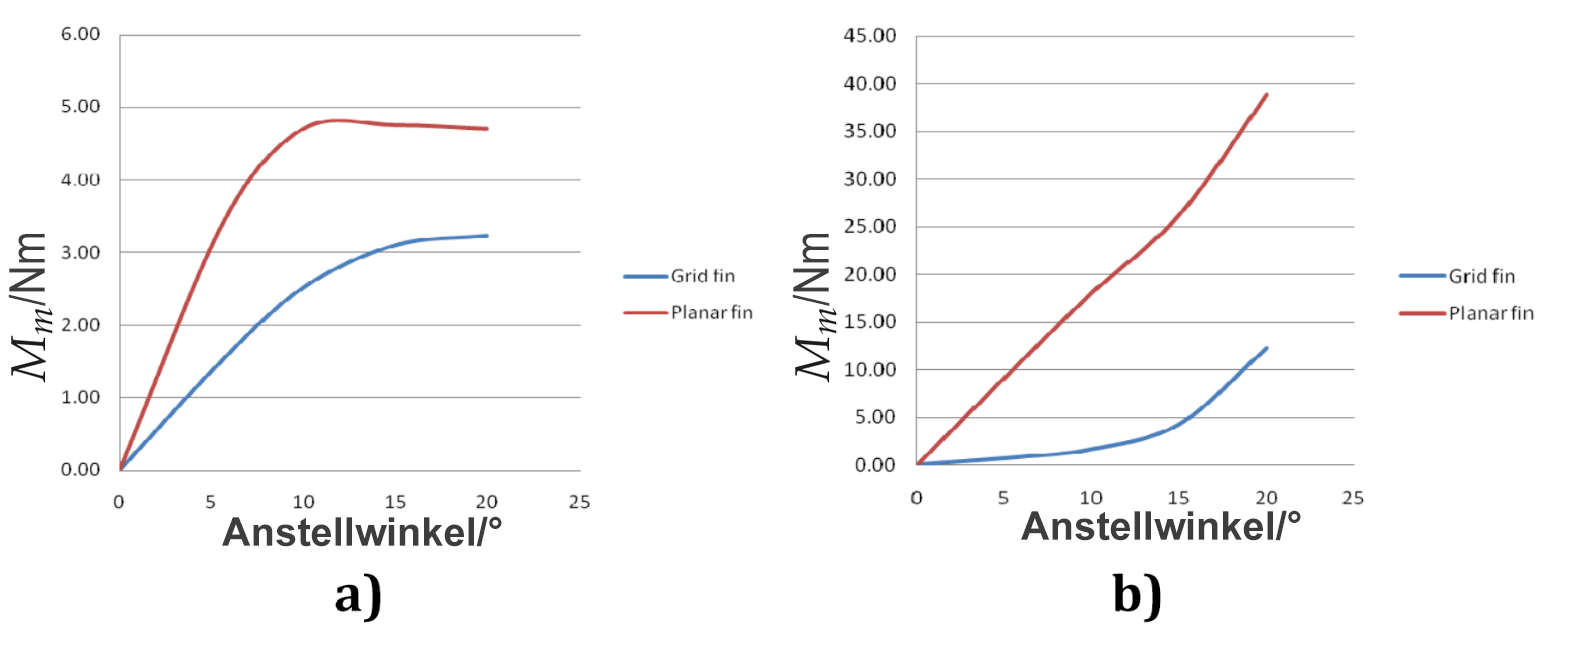
\includegraphics[width=0.8\textwidth]{gelenkmoment.png}
	\caption{Gelenkmoment über Anstellwinkel bei a) \ensuremath{Ma=0,5}, b) $Ma=2,5$ aus \cite{vergleichPlanar}}
	\label{abb_Mm-AoA}
\end{figure}


\subsection{Grid Fin Varianten}
Bisher wurde nur eine sehr simple Version von Grid Fins betrachtet. Es gibt jedoch eine Vielzahl von Variationen, die genutzt werden können, um die aerodynamischen Eigenschaften für bestimmt Anwendungen zu optimieren. In diesem Abschnitt werden einige Möglichkeiten beschrieben, wie diese unkonventionellen Finnen angepasst werden können eingegangen.
\subsubsection{Pfeilung}
Eine Häufige Kritik von Grid Fins sind ihre hohen Axial- bzw. Widerstandskräfte. Somit ist es nicht verwunderlich, dass ein Großteil von Studien sich auf die Reduzierung dieses Aspektes konzentriert haben. Eine Häufig gewählte Methode ist hierbei die Pfeilung, deren Nutzen aus den planaren Tragflächentechnik schon seit längerer Zeit bekannt ist. Es wird in dieser Arbeit jedoch zwischen drei verschiedenen Varianten unterschieden, wie sich diese Pfeilung auf die komplexe Gitterstruktur übertragen lässt.\\
~\\
Die erste Variante stellt die \textbf{Pfeilung der gesamten Konfiguration} dar. Hierbei beleibt der Grid Fin an sich ungepfeilt. Stattdessen wird die Pfeilung dadurch erreicht, dass die Querschnittfläche nicht senkrecht zur Oberfläche des Flugkörpers steht. Sie ist um den Pfeilungswinkel $\Lambda_{\gls{Index:Konf}}$, welcher identisch mit dem Klappwinkel $\Lambda$ ist, geneigt. Dass der Pfeilungswinkel dem Klappwinkel entspricht, zeigt direkt einen Vorteil dieser Variante. Der Pfeilungswinkel kann während des Einsatzes verstellt und den Strömungsbedingungen und Anforderungen der Flugphase angepasst werden.\\
Der Effekt ist hier aber nicht eine Reduzierung des Widerstandes, ganz im Gegenteil. Die Pfeilung erhöht die Axialkraft, sodass sie bei einem Winkel von $\Lambda_{Konf} = \pm45^\circ$ ein neues Maximum erreicht. Hierbei bewirkt die Vorwärtspfeilung, negativer Winkel, sogar $10\%$ mehr, als die Rückwärtspfeilung \cite{LambdaKonf}. Im Unterschall kann somit eine Axialkraftsteigerung mit dem Faktor 5, Faktor 3 im Transschall und im Überschall bei $Ma = 2,5$ wiederum Faktor 4 erreicht werden \cite{LambdaKonf}. Zusätzlich ist die Axialkraft bei Pfeilungswinkel $\Lambda_{Konf} \neq 0$ und hohen Machzahlen nicht mehr konstant, sondern steigt noch weiter an.

Die Normalkraftgenerierung ist jedoch auch reduziert. Bei maximaler Axialkraft beträgt die Normalkraft 30\% bis 50\% weniger also ohne Pfeilung. Bei kleinen Winkeln bis zu $\Lambda_{Konf} = \pm20^\circ$ ist dieser Einfluss jedoch noch vernachlässigbar.

Eine Pfeilung der Konfiguration lässt also flexibel das Potenzial der Grid Fins zur Anwendung als Drag Brakes anpassen. Auch wenn für eine maximale Axialkraft die Steuerbarkeit stark beeinträchtigt wird, kann, wenn der Bedarf an Widerstand es zulässt, bei kleinen Pfeilungswinkel weiterhin reguläre Beträge an Normalkraft generiert werden.
\begin{figure}[h]
	\centering
	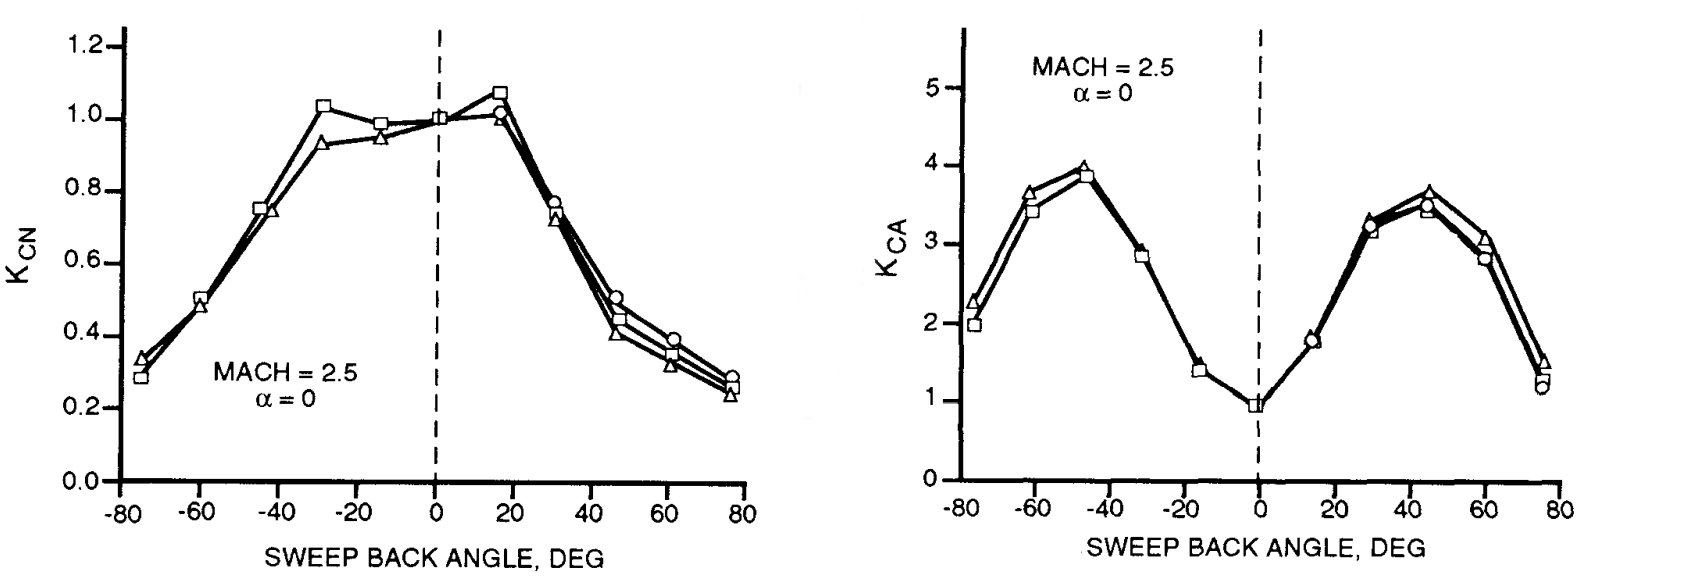
\includegraphics[width=\textwidth]{PfeilKonf.png}
	\caption{Vielfache des Normalkraftanstiegs (links) und der Axialkraft (rechts) im Vergleich zum ungepfeilten Grid Fin über konfigurellen Pfeilungswinkel $\Lambda_{Konf}$ bei $Ma = 2,5$ und $\alpha = 0$ aus \cite{LambdaKonf}}
\end{figure}

Die zweite Variante ist eine \textbf{Pfeilung des Gitters} entlang der Steuerachse, sodass die auf die Y-Z-Ebene projizierte Geometrie unverändert bleibt. Das Ziel hierbei ist es die Axialkraft zu senken, indem die Verdichtungsstöße an den Gittervorderkanten nicht alle auf derselben Höhe liegen, sondern in X-Richtung gestaffelt stattfinden.
\begin{figure}[h]
	\centering
	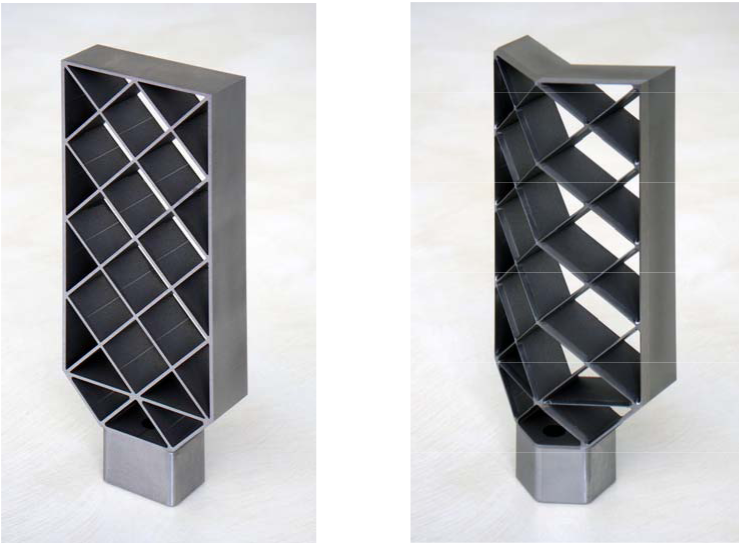
\includegraphics[width=0.6\textwidth]{PfeilGBild.png}
	\caption{Ebener Grid Fin (links) und Grid Fin mit gepfeiltem Gitter (rechts) aus \cite{PfeilG3}}
\end{figure}\\
Mit steigender Pfeilung des Gitters $\Lambda_G$ wächst die effektive Länge der Zellen, die als Düse fungieren. Der Stoß befindet sich somit näher an der Vorderkante und besitzt einen geringeren Winkel. Dies reduziert die Drosselung und die Expansionswellen am Zellausgang nehmen ab \cite{PfeilG1}. Dies sorgt dafür, dass im Bereich der kritischen Machzahlen die Axialkraft deutlich verringert wird. Auch der Gradient der Normalkraft $F_N\alpha$ nimmt mit steigenden Pfeilungswinkel im transsonischen Bereich zu \cite{PfeilG1}, was die Stabilität deutlich erhöht. Eine Vorwärtspfeilung $\Lambda_{G} < 0$ zeigt grundsätzlich ähnliche wenn auch schwächere Effekt wie die Rückwärtspfeilung \cite{PfeilG2}. Im Überschall wird der Effekt auf die Axialkraft ab, sodass er vernachlässigbar wird. Für die Normalkraftgenerierung dreht sich die Wirkung der Pfeilung bei diesen Machzahlen sogar um, sodass schon bei $Ma=2$ der ungepfeilte Grid Fin den gepfeilten überlegen ist.

Eine Pfeilung des Gitters birgt also hauptsächlich für den Transschall Vorteile wie geringere Axialkraft und einen erhöhten Normalkraftanstieg. Bei höheren Machzahlen bewirkt die Pfeilung jedoch auch bei letzterem eine Senkung, wodurch die Stabilität im Überschall reduziert wird.
\begin{figure}[h]
	\centering
	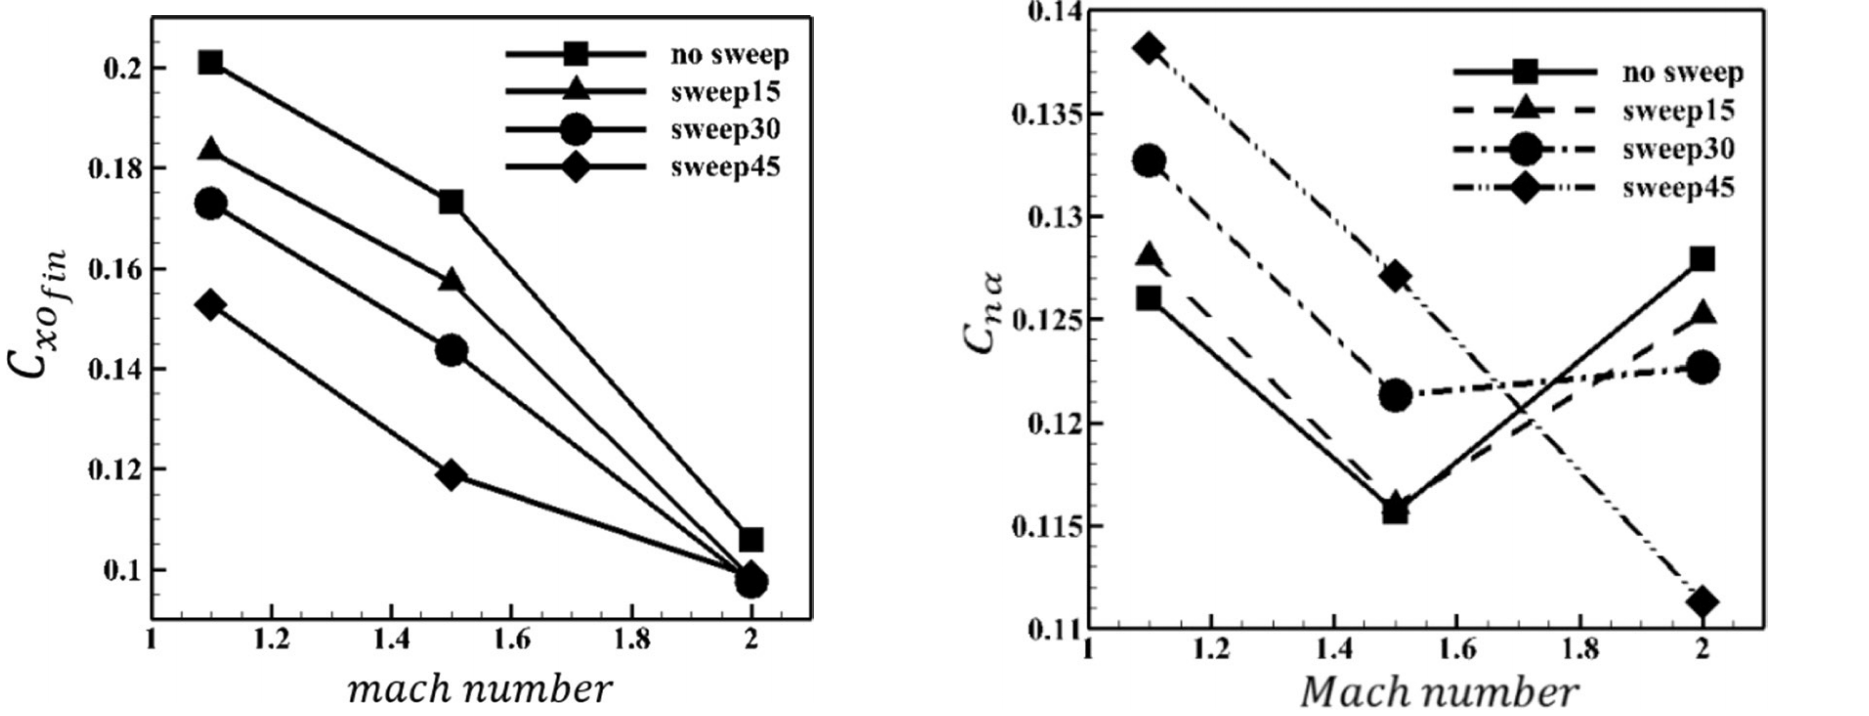
\includegraphics[width=\textwidth]{PfeilG_Ma.png}
	\caption{Axialkraftbeiwert (links) und Normalkraftsbeiwertanstieg (rechts) über die Machzahl bei unterschiedlichen Pfeilungswinkeln $\Lambda_{G}$ bei $\alpha = 0$ aus \cite{PfeilG1}}
\end{figure}\\
Als letzte Variante bleibt die \textbf{lokale Pfeilung der einzelnen Zellen} übrig. Die Zellwände kann man sich hierbei wie nebeneinander gereihte Deltaflügel vorstellen, sodass die luv-Seite des Grid Fins mit Zacken übersät ist. Für die Beschreibung dieser Pfeilung wird nicht nur der Winkel $\Lambda_{\gls{Index:Z}}$, sondern auch die Anzahl der Zahn pro Zelle und ihre Position relativ zu den Schnittstellen des Gitters, benötigt. Im Folgenden wird nur der Fall einem Zahn zwischen zwei Schnittstellen der Zellwände betrachtet. Für die Position der Spitze werden zwei Typen unterschieden. Beim Tal-Typus befindet sich die Spitze in der Mitte der Zellwand, sodass sich an der Schnittstelle alle sich kreuzende Zellwände ein "Tal"\ teilen. Der Berg-Typus hingegen hat ein Tal in der Mitte und benachbarte Zellen teilen sich einen "Berg".
Die folgenden Eigenschaften beziehen sich auf ein Gitter, deren Vorder- und Hinterkanten nicht wie bisher betrachtet stumpf, sondern zugespitzt sind. Auf unterschiedliche Kantenformen wird später in diesem Kapitel noch eingegangen. 
\begin{figure}[h]
	\centering
	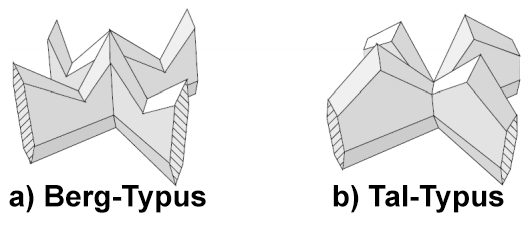
\includegraphics[width=0.6\textwidth]{PeakValley.png}
	\caption{Lokale Pfeilung der Zelle mit dem a) \grqq Berg\grqq -Typus und b) \grqq Tal\grqq -Typus aus \cite{PeakValley}}
\end{figure}\\
Trifft nun eine Strömung auf lokal gepfeilte Gitterwände, so bilden sich an der Vorderkante drei verschiedene Druckbereiche. An der Spitze und von dort aus im Machkegel strömungsabwärts befindet sich eine 2D-Strömung, in deren Gebiet ein geringerer Druck an der Oberfläche herrscht. Im Tal hingegen kommt es zu deutlich erhöhtem Druck, da die Schockwellen der Pfeilung folgen und sich somit die der benachbarten Zähne hier kreuzen. Während die Größe dieser beiden Zonen relativ unabhängig von der Zahngröße ist, wachsen und schrinken die Ausmaße des Bereiches mit abgeschwächter Wellenintensität zwischen ihnen mit ihr \cite{PeakValley}.

Wird nun zuerst eine einzelne planare Wand unendlicher Streckung mit lokaler Pfeilung betrachtet, so zeigt sich eine Abnahme der Axialkraft mit steigenden Pfeilungswinkel $\Lambda_Z$ \cite{PeakValley}. Je hoher die Machzahl, dicker die Wandstärke und stumpfer die Vorderkante ist, desto stärker macht sich der Effekt bemerkbar. Im Gegensatz dazu verringert die Zahnlänge und der Anstellwinkel die Effektivität der lokalen Pfeilung \cite{PeakValley}.

Auch beide Typen von lokaler Pfeilung am Gitter reduzieren den Wellenwiderstand deutlich. Bei Tal-Typus treffen jedoch vier statt nur zwei Wellen aufeinander, sodass es zu größeren Verlusten kommt und die Widerstandsreduzierung beim Berg-Typus bei einer Machzahl von $Ma=6$ um $1,2\%$ stärker ist \cite{PeakValley}.
Wie in Abbildung \ref{abb_PeakValley-Ma} zu sehen haben lokal gepfeilte Grid Fins auch ein höheres Auftrieb zu Widerstand Verhältnis, jedoch ist ihr Vorteil hier geringer, als beim Widerstand sodass ein geringerer Auftrieb vorliegen muss. Zusätzlich zeigt an dieser Stelle der Tal-Typus bessere Eigenschaften, da seine Auftriebserzeugung über der des Berg-Typus liegt. 
\begin{figure}[h]
	\centering
	\includegraphics[width=0.9\textwidth]{PeakValley_Cd-Ma.png}
	\caption{Widerstandsbeiwert (links) und Auftrieb/Widerstand-Verhältnis (rechts) über Machzahl aus \cite{PeakValley}}
	\label{abb_PeakValley-Ma}
\end{figure}\\
Bei hohen Machzahlen lässt sich nun also mittels der lokalen Pfeilung der einzelnen Zellen, die Axialkraft auf Grid Fins stark vermindern. Dabei müssen jedoch leichte Einbußen im Bezug auf die Normalkraft in Kauf genommen werden.
\subsubsection{Krümmung}
Um das Transportpotenzial von Grid Fins am besten nutzen zu können, ist es wünschenswert, dass sie sich im eingeklappten Zustand an den Körper anschmiegen. Somit hätten sie, je nachdem ob sie in Flugrichtung ($\Lambda = -90^\circ$) oder entgegen ($\Lambda = 90^\circ$) gedreht werden, eine konkave oder konvexe Krümmung zur Anströmung, deren Radius dem vom Körper entspricht.

Dies hat unabhängig der Ausrichtung der Krümmung nur einen geringen Einfluss auf die Aerodynamik. Weder Axial- noch Normalkraft zeigen signifikante Änderungen \cite{LambdaKonf}, sodass die Leistungsfähigkeit erhalten bleibt. Beim Gelenkmoment zeichnen sich jedoch Unterschiede ab. Die konvexe Krümmung führt zu einem sehr kleinen Moment, dass sich für Anstellwinkel zwischen $\alpha = -10^\circ$ und $\alpha=20^\circ$ um die null bewegt \cite{LambdaKonf}. Für den konkaven Grid Fin zeigt sich jedoch ein Anstieg des Gelenkmomentes mit dem Anstellwinkel, der steiler ist als der des flachen \cite{LambdaKonf}. Hier sei jedoch anzumerken, dass sich die Werte noch immer in einem sehr niedrigen Bereich deutlich unter planaren Finnen bewegen.

Somit lässt sich mit einer Krümmung des Grid Fins, die der des Flugkörpers entspricht, die Transportmöglichkeiten ideal nutzen, ohne spürbare Einbußen in der Leistung zu haben.
\subsubsection{Kanten}

\subsubsection{Zellform}
Für die Form der einzelnen Zellen sind unterschiedliche Varianten denkbar. Neben Rechtecken sind auch Dreiecke möglich, welche der Struktur eine noch höhere Stabilität verleihen. Alternativ wäre für den idealen Durchlass der Strömung eine runde Zelle am besten. Um damit ein Gitter lückenlos füllen zu können, kann hier auf eine bienenwabenähnliche Sechseckstruktur zurück gegriffen werden \cite{Pattern}. In Abbildung \ref{abb_parameter} ist auch schon eine Kombination unterschiedlich geformter Zellen zu sehen, was eine flexible Gestaltung der Gesamtgitterform ermöglicht.\\


\section{Bisherige Implementierung}


\section{Wiedereintrittsbedingungen}


\section{Das Air-Launchsystem Valkyrie}

